
While solving the heat balance equation related to the quench propagation, the solver must handle high nonlinearities of material properties at cryogenic temperatures. In a problem of this kind, the material properties are locally linearised. The solver iterates over the temperature distribution in space until the change of temperature between two consecutive iterations converges to a desirably low value. In order to accurately solve the temperature distribution in the entire region of the cable, one should locally refine mesh in the occurrence of a high temperature difference and/or decrease the simulation time step (up to the order of a $\upmu$s).

Figure~\ref{fig:modelling_approach} presents an approximated temperature distribution over a discretised 1D thermal domain. The quenched and non-quenched regions in a superconducting cable have different, but relatively uniform, temperature distribution except for the regions close to the quench front. Therefore, in a general analysis of the quench propagation, the mesh density relatively far from the quench front can be relaxed due to the lower temperature difference between the nodes. 

\begin{figure}[H]
\centering
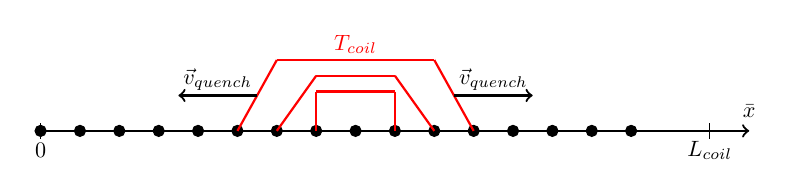
\begin{tikzpicture}[scale = 1]
\draw [thick, ->] (0.0,0.0) -- (9.0,0);
\foreach \t in {0,0.5,1,...,7.5}
\filldraw[black] ({\t},0) circle (2pt);
\draw [thick, red] (3.5,0) -- (3.5,0.5);
\draw [thick, red] (3.5,0.5) -- (4.5,0.5);
\draw [thick, red] (4.5,0.5) -- (4.5,0);
\draw [thick, red] (3,0) -- (3.5,0.7);
\draw [thick, red] (3.5,0.7) -- (4.5,0.7);
\draw [thick, red] (4.5,0.7) -- (5,0);
\draw [thick, red] (2.5,0) -- (3,0.9);
\draw [thick, red] (3,0.9) -- (5,0.9);
\draw [thick, red] (5,0.9) -- (5.5,0);
\draw [thick, ->] (5.25,0.45) -- (6.25,0.45);
\node[scale = 0.8] at (5.75,0.65) {$\vec{v}_\text{quench}$};
\draw [thick, ->] (2.75,0.45) -- (1.75,0.45);
\node[scale = 0.8] at (2.25,0.65) {$\vec{v}_\text{quench}$};
\node[scale = 0.8, red] at (4,1.1) {$T_\text{coil}$};

\node[scale = 0.8] at (9.0,+0.25) {$\bar x$};
\node[scale = 0.8] at (8.5,-0.25) {$L_\text{coil}$};
\draw [thin] (8.5,-0.10) -- (8.5,0.10);
\draw [thin] (0,-0.10) -- (0,0.10);
\node[scale = 0.8] at (0,-0.25) {0};

\end{tikzpicture}
\caption{Schematic of the temperature propagation with quench velocity modelling.}
\label{fig:modelling_approach}
\end{figure}

While solving the quench propagation by means of the quench velocity-based approach, a constant quench velocity along a given winding (subject to local magnetic field) is assumed. The quench velocity is integrated over time in an external routine and assigned to a thermal model as a quench front position. As a result of providing the quench position over time, the mesh refinement along the coil (also at the quench front) is no longer required and the numerical model with less degrees of freedom is solved. In other words, the numerical model still calculates the heat balance equation, but with a fixed and relatively coarse mesh along the entire strand. The temperature distribution close to the quench front is approximated, knowing that it is placed between two extreme temperatures (either inside or outside of the quenched zone).
